%%%%%%%%%%%%%%%%%%%%%%%%%%%%%%%%%%%%% 
% Check out the accompanying book, Even Better Books with LaTeX the Agile Way in 2023, for a discussion of the template and step-by-step instructions. https://amzn.to/3HqwgXM https://leanpub.com/eBBwLtAW/
% The template was originally created by Clemens Lode, LODE Publishing (www.lode.de), on 1/1/2023. Feel free to use this template for your book project! 
% I would be happy if you included a short mention in your book in order to help others to create their own books, too ("Book template based on \textit{Even Better Books with LaTeX the Agile Way in 2023} by Clemens Lode").
% Contact me at mail@lode.de if you need help with the template or are interested in our editing and publishing services.
% And don't forget to follow us on Instagram! https://www.instagram.com/lodepublishing/ https://www.instagram.com/betterbookswithlatex/
%%%%%%%%%%%%%%%%%%%%%%%%%%%%%%%%%%%%%

% To create an EPUB file, select pdfLaTeX in the Menu in the top-left and choose the conversion method in the /latexmkrc file.

% Select document class scrbook to be in the two-page mode and accommodate for the binding of a printed book.
% The bibliography receives an entry in the table of contents but no number.
\documentclass[pagesize=auto,bibliography=totocnumbered]{scrbook}

%%%%%%%%%%%%%%%%%%%%%%%%%%%%%%%%%%%%% 
% Check out the accompanying book, Even Better Books with LaTeX the Agile Way in 2023, for a discussion of the template and step-by-step instructions. https://amzn.to/3HqwgXM https://leanpub.com/eBBwLtAW/
% The template was originally created by Clemens Lode, LODE Publishing (www.lode.de), on 1/1/2023. Feel free to use this template for your book project! 
% I would be happy if you included a short mention in your book in order to help others to create their own books, too ("Book template based on \textit{Even Better Books with LaTeX the Agile Way in 2023} by Clemens Lode").
% Contact me at mail@lode.de if you need help with the template or are interested in our editing and publishing services.
% And don't forget to follow us on Instagram! https://www.instagram.com/lodepublishing/ https://www.instagram.com/betterbookswithlatex/
%%%%%%%%%%%%%%%%%%%%%%%%%%%%%%%%%%%%%

% Replace "The Title" with your book title.
\newcommand{\mytitle}{The Title}

% Replace "The subtitle" with your book's subtitle.
\newcommand{\mysubtitle}{The subtitle}

% Replace "Publishing Company" with the name of the publishing company it is published.
\newcommand{\mypublishingcompany}{Publishing Company}

% Replace "Location of the Publishing Company (city)" with the location (e.g., the city) of the publishing company.
\newcommand{\mypublishingcompanylocation}{Location of the Publishing Company (city)}

\newcommand{\mypublishingcompanyurl}{\url{https://www.lode.de}}


% Upload a low-resolution jpg (e-book) and a high-resolution (pdf/print) png version of your front cover into the "images" folder. If you need help with creating a cover, email us at mail@lode.de to talk about what you need, and we will do our best to help you.
\newcommand{\coverImage}{images/cover.jpg}
\newcommand{\hiresCoverImage}{images/cover.png}


% Replace "Your email address" with your email address.
% Replace "Edition" with the edition number.
% Replace the ISBNs with your ISBNs. 
% Replace "Your editor's name" with your editor's name.
% Replace "Your designer's name" with your book cover designer's name.
% Replace "Your image sources" with the sources of your images (including icons) and relevant license information.
% Replace "Your newsletter email" with your newsletter email.
% Replace "Your newsletter URL" with your website's newsletter URL.


\newcommand{\mypublishingcompanyemail}{Your email address}
\newcommand{\editionNumber}{First}

% Buy ISBNs or use the ISBNs generated by Amazon and list them  here.
\newcommand{\ebookISBN}{123-4-567890-12-3}
\newcommand{\softcoverISBN}{123-4-567890-12-4}
\newcommand{\hardcoverISBN}{123-4-567890-12-5}

\newcommand{\editorName}{Your editor's name}
\newcommand{\designerName}{Your designer's name}
\newcommand{\imageSources}{Your image sources}

\newcommand{\newsletterMail}{Your newsletter email}
\newcommand{\newsletterURL}{Your newsletter URL}

% If you want to subscribe to this book's newsletter, write an email to newsletter@lode.de or follow us on Instagram.com/lodepublishing or Instagram/betterbookswithlatex

\newcommand{\yourName}{Your name}

% Replace city, country, and date with the place and country where you (or your company) are located and the date when the preface was finished (it does not have to be the release date of the book).

\newcommand{\yourCity}{Your city}
\newcommand{\yourCountry}{Your country}
\newcommand{\prefaceDate}{Preface date}

\newif\ifuseAuthorImage
% Uncomment and upload author images
%\useAuthorImagetrue

\ifuseAuthorImage
    \newcommand{\authorImage}{images/author.jpg}
    \newcommand{\authorImageHiRes}{images/author.png}
\fi


% Uncomment \seriestrue if your book is part of a series.
\newif\ifseries
%\seriestrue

\ifseries
% Replace "Title of Book Series" with the title of the book series.
% Replace "Title of Part One" with the title of part one.
% Replace "Title of Part Two" with the title of part two.
% Replace "Title of Part Three" with the title of part three, or remove the line if there is no part three.
% Replace "Title of Part Four" with the title of part four, or remove the line if there is no part four.

\newcommand{\partOneTitle}{Title of Part One}
\newcommand{\partTwoTitle}{Title of Part Two}
\newcommand{\partThreeTitle}{Title of Part Three}
\newcommand{\partFourTitle}{Title of Part Four}

\newcommand{\titleOfTheBookSeries}{Title of the Book Series}

\newif\firstBookOfSeries
\firstBookOfSeries

\ifFirstBookOfSeries
\else
\newcommand{\partPreviousPart}{Number of the previous part in the book series}
\newcommand{\titlePreviousPart}{Title of the previous part in the book series}

\newcommand{\previousCoverImage}{images/previous_part_of_the_series_Cover.jpg}
\newcommand{\previousCoverImageHiRes}{images/previous_part_of_the_series_Cover_hires.png}

\fi


% If you want a different size than 6"x9", change the lib/bookformat.tex file accordingly.

\newif\ifhardcover
% Uncomment for selecting hardcover.
%\hardcovertrue
\title{\mytitle}

% Load additional LaTeX libraries.
%%%%%%%%%%%%%%%%%%%%%%%%%%%%%%%%%%%%% 
% Check out the accompanying book, Even Better Books with LaTeX the Agile Way in 2023, for a discussion of the template and step-by-step instructions. https://amzn.to/3HqwgXM https://leanpub.com/eBBwLtAW/
% The template was originally created by Clemens Lode, LODE Publishing (www.lode.de), on 1/1/2023. Feel free to use this template for your book project! 
% I would be happy if you included a short mention in your book in order to help others to create their own books, too ("Book template based on \textit{Even Better Books with LaTeX the Agile Way in 2023} by Clemens Lode").
% Contact me at mail@lode.de if you need help with the template or are interested in our editing and publishing services.
% And don't forget to follow us on Instagram! https://www.instagram.com/lodepublishing/ https://www.instagram.com/betterbookswithlatex/
%%%%%%%%%%%%%%%%%%%%%%%%%%%%%%%%%%%%%



% This configures the PDF/EPUB output.
%%%%%%%%%%%%%%%%%%%%%%%%%%%%%%%%%%%%% 
% Check out the accompanying book, Even Better Books with LaTeX the Agile Way in 2023, for a discussion of the template and step-by-step instructions. https://amzn.to/3HqwgXM https://leanpub.com/eBBwLtAW/
% The template was originally created by Clemens Lode, LODE Publishing (www.lode.de), on 1/1/2023. Feel free to use this template for your book project! 
% I would be happy if you included a short mention in your book in order to help others to create their own books, too ("Book template based on \textit{Even Better Books with LaTeX the Agile Way in 2023} by Clemens Lode").
% Contact me at mail@lode.de if you need help with the template or are interested in our editing and publishing services.
% And don't forget to follow us on Instagram! https://www.instagram.com/lodepublishing/ https://www.instagram.com/betterbookswithlatex/
%%%%%%%%%%%%%%%%%%%%%%%%%%%%%%%%%%%%%

% This command enables checking if XeLaTeX is used.
\usepackage{ifxetex}

\ifxetex
    % For the PDF output, load the following additional packages.
    
    % This adjusts figures to fit into the width of a page.
    \usepackage{adjustbox}
    
    % Use this for fancy lines at the beginning of chapters and the end of sections.
    \usepackage{psvectorian} 

\else
    % Ignore adjustbox commands (HTML files do not have a width).
    \newcommand{\adjustbox}[2][]{#1}

    % Ignore psvectorian lines.
    \newcommand{\psvectorian}[2][]{}
\fi

% Translate newpage and hrule commands.
\ifx\HCode\undefined
    \newcommand{\nextpage}[1][]{}
\else
    \newcommand{\nextpage}[1][]{\HCode{<mbp:pagebreak />}}
    \renewcommand{\hrule}{\HCode{<hr style="clear: both" />}}
\fi

% Sets up support for multiple languages.
%%%%%%%%%%%%%%%%%%%%%%%%%%%%%%%%%%%%% 
% Check out the accompanying book, Even Better Books with LaTeX the Agile Way in 2023, for a discussion of the template and step-by-step instructions. https://amzn.to/3HqwgXM https://leanpub.com/eBBwLtAW/
% The template was originally created by Clemens Lode, LODE Publishing (www.lode.de), on 1/1/2023. Feel free to use this template for your book project! 
% I would be happy if you included a short mention in your book in order to help others to create their own books, too ("Book template based on \textit{Even Better Books with LaTeX the Agile Way in 2023} by Clemens Lode").
% Contact me at mail@lode.de if you need help with the template or are interested in our editing and publishing services.
% And don't forget to follow us on Instagram! https://www.instagram.com/lodepublishing/ https://www.instagram.com/betterbookswithlatex/
%%%%%%%%%%%%%%%%%%%%%%%%%%%%%%%%%%%%%

% Activate American language (and \babelEN).
\usepackage[american]{babel}

% Activate German language (and \babelDE).
%\usepackage[ngerman]{babel}

% Fix PDF creation.
\ifxetex
	\let\pdfstrcmp\strcmp
\fi
% Set up macros to support multiple languages:
\newcommand{\babelDE}[1]{\ifnum\pdfstrcmp{\languagename}{ngerman}=0 {#1}\fi}
\newcommand{\babelEN}[1]{\ifnum\pdfstrcmp{\languagename}{american}=0 {#1}\fi}

% Loads packages to be able to configure hyphenation.
%%%%%%%%%%%%%%%%%%%%%%%%%%%%%%%%%%%%% 
% Check out the accompanying book, Even Better Books with LaTeX the Agile Way in 2023, for a discussion of the template and step-by-step instructions. https://amzn.to/3HqwgXM https://leanpub.com/eBBwLtAW/
% The template was originally created by Clemens Lode, LODE Publishing (www.lode.de), on 1/1/2023. Feel free to use this template for your book project! 
% I would be happy if you included a short mention in your book in order to help others to create their own books, too ("Book template based on \textit{Even Better Books with LaTeX the Agile Way in 2023} by Clemens Lode").
% Contact me at mail@lode.de if you need help with the template or are interested in our editing and publishing services.
% And don't forget to follow us on Instagram! https://www.instagram.com/lodepublishing/ https://www.instagram.com/betterbookswithlatex/
%%%%%%%%%%%%%%%%%%%%%%%%%%%%%%%%%%%%%

% Use fontenc to properly hyphenate accented languages.
\usepackage[T1]{fontenc}

% Add a list of words to enforce a certain hyphenation for them.
\usepackage{hyphenat}
\hyphenation{}



% In this package, we define the dimensions of the printed book.
%%%%%%%%%%%%%%%%%%%%%%%%%%%%%%%%%%%%% 
% Check out the accompanying book, Even Better Books with LaTeX the Agile Way in 2023, for a discussion of the template and step-by-step instructions. https://amzn.to/3HqwgXM https://leanpub.com/eBBwLtAW/
% The template was originally created by Clemens Lode, LODE Publishing (www.lode.de), on 1/1/2023. Feel free to use this template for your book project! 
% I would be happy if you included a short mention in your book in order to help others to create their own books, too ("Book template based on \textit{Even Better Books with LaTeX the Agile Way in 2023} by Clemens Lode").
% Contact me at mail@lode.de if you need help with the template or are interested in our editing and publishing services.
% And don't forget to follow us on Instagram! https://www.instagram.com/lodepublishing/ https://www.instagram.com/betterbookswithlatex/
%%%%%%%%%%%%%%%%%%%%%%%%%%%%%%%%%%%%%

%%%%%%%%%%%%%%%%%
% Configure bleed.
%%%%%%%%%%%%%%%%%

% If your book includes images that extend beyond the usual margins, set bleed to 0.125in and activate the corresponding option in Amazon KDP.

\newcommand{\bleed}{0in}
%\newcommand{\bleed}{0.125in}

\newcommand{\margintop}{0.3in}
\newcommand{\marginbottom}{0.3in}
\newcommand{\marginoutside}{0.3in}

%%%%%%%%%%%%%%%%%
% The inner margins depend on the number of pages of your book. 
%%%%%%%%%%%%%%%%%

% Note that books printed by Amazon have an upper limit of number of pages. This limits depends on your book's dimensions, whether it is a paperback or hardcover format, and whether it is printed in black and white or in color.
% See https://kdp.amazon.com/en_US/help/topic/GVBQ3CMEQW3W2VL6

% Select the margin for 24 - 150 pages by default.
\newcommand{\margininside}{0.425in}
% 151 - 300 pages
%\newcommand{\margininside}{0.55in}
% 301 - 500 pages
%\newcommand{\margininside}{0.675in}
% 501 - 700 pages
%\newcommand{\margininside}{0.8in}
% 701 - 828 pages
%\newcommand{\margininside}{0.925in}


%%%%%%%%%%%%%%%%%
% Hardcover / Softcover Formats. Selecting one of these ensures that you can use the same PDF for hardcover and softcover books on Amazon.
%%%%%%%%%%%%%%%%%

%\newcommand{\bookwidth}{5.5in}\newcommand{\bookheight}{8.5in}
% Select 6"x9" by default.
\newcommand{\bookwidth}{6in}\newcommand{\bookheight}{9in}
%\newcommand{\bookwidth}{6.14in}\newcommand{\bookheight}{9.21in}
%\newcommand{\bookwidth}{7in}\newcommand{\bookheight}{10in}

%%%%%%%%%%%%%%%%%
% Hardcover-only formats. Selecting one of these requires you to create a separate PDF for a softcover version.
%%%%%%%%%%%%%%%%%

%\newcommand{\bookwidth}{8.25in}\newcommand{\bookheight}{11in}

%%%%%%%%%%%%%%%%%
% Softcover-only formats. Selecting one of these requires you to create a separate PDF for a hardcover version.
%%%%%%%%%%%%%%%%%

%\newcommand{\bookwidth}{5in}\newcommand{\bookheight}{8in}
%\newcommand{\bookwidth}{5.25in}\newcommand{\bookheight}{8in}
%\newcommand{\bookwidth}{5.06in}\newcommand{\bookheight}{7.81in}
%\newcommand{\bookwidth}{6.69in}\newcommand{\bookheight}{9.61in}
%\newcommand{\bookwidth}{7.44in}\newcommand{\bookheight}{9.69in}
%\newcommand{\bookwidth}{7.5in}\newcommand{\bookheight}{9.25in}
%\newcommand{\bookwidth}{8in}\newcommand{\bookheight}{10in}
%\newcommand{\bookwidth}{8.5in}\newcommand{\bookheight}{11in}

%%%%%%%%%%%%%%%%%
% And now we are putting everything together to set the dimensions of the book.
%%%%%%%%%%%%%%%%%

\usepackage[paperwidth=\dimexpr\bookwidth+\bleed\relax, paperheight=\dimexpr\bookheight+\bleed+\bleed\relax, inner=\margininside, outer=\dimexpr\marginoutside+\bleed\relax, top=\dimexpr\margintop+\bleed\relax, bottom=\dimexpr\marginbottom+\bleed\relax,includehead, includefoot, headheight=32pt]{geometry}

% This package defines all the box commands.
%%%%%%%%%%%%%%%%%%%%%%%%%%%%%%%%%%%%% 
% Check out the accompanying book, Even Better Books with LaTeX the Agile Way in 2023, for a discussion of the template and step-by-step instructions. https://amzn.to/3HqwgXM https://leanpub.com/eBBwLtAW/
% The template was originally created by Clemens Lode, LODE Publishing (www.lode.de), on 1/1/2023. Feel free to use this template for your book project! 
% I would be happy if you included a short mention in your book in order to help others to create their own books, too ("Book template based on \textit{Even Better Books with LaTeX the Agile Way in 2023} by Clemens Lode").
% Contact me at mail@lode.de if you need help with the template or are interested in our editing and publishing services.
% And don't forget to follow us on Instagram! https://www.instagram.com/lodepublishing/ https://www.instagram.com/betterbookswithlatex/
%%%%%%%%%%%%%%%%%%%%%%%%%%%%%%%%%%%%%

% Replace the "Did you know?", "Read more in...", box titles, and icons if necessary.

% Configuring the commands for the PDF output...
\ifx\HCode\undefined 

    % If you want to add a picture to the top right corner of a box, uncomment the line and upload the picture.

    \usepackage[many]{tcolorbox}
    
    \newtcolorbox{problem}[1][]{colframe = black!30,colback  = black!4,coltitle = black!20!black,title=\babelDE{\textbf{Frage}}\babelEN{\textbf{Question}}
    %\hfill\smash{\raisebox{-11pt}{\includegraphics[height=1cm]{images/speech-bubble-cloud-with-question-mark.png}}}
    , #1,}
    
    \newtcolorbox{idea}[1][]{colframe = black!30,colback  = black!5,coltitle = black!30!black,title=\babelDE{\textbf{Idee}}\babelEN{\textbf{Idea}}
    %\hfill\smash{\raisebox{-11pt}{\includegraphics[height=1cm]{images/lightbulb-idea}}}
    , #1,}

    \newtcolorbox{example}[1][]{colframe = black!20,colback  = black!0,coltitle = black!20!black,title=\babelDE{\textbf{Beispiel}}\babelEN{\textbf{Example}}
    %\hfill\smash{\raisebox{-11pt}{\includegraphics[height=1cm]{images/book-and-test-tube-with-supporter}}}
    , #1,}

    
    \newtcolorbox{biography}[2][]{colframe = black!30,colback  = black!5,coltitle = black!30!black,title=\babelDE{Biographie -- }\babelEN{Biography---}\textbf{#2}
    %\hfill\smash{\raisebox{-11pt}{\includegraphics[height=1cm]{images/identity-card}}}
    , #1,}
    
% ... and for the HTML output.
\else
	
    \newenvironment{problem}[1][]{\bfseries\HCode{<b>}}{\HCode{</b>}\par}
    
    \newenvironment{idea}[1][]{\bfseries\HCode{<b>}}{\HCode{</b>}\par}
	
    \newenvironment{example}[1][]{\hrule\par \textbf{\babelDE{Beispiel}\babelEN{Example}}\par}{\hrule\par}
    
    \newenvironment{biography}[2][]{\hrule\par\textbf{\babelDE{Biographie}\babelEN{Biography}} \emdash \textbf{#2}\par}{\hrule\par}

\fi



% Print out listings as-is (ignoring any special characters).
\usepackage{listings}




\ifx\HCode\undefined 

% This code loads the \leftbar command for the definition environment.
    \usepackage{framed}
    \newenvironment{definition}[2][]{\begin{leftbar}\textbf{\textsc{#2}}\ ·\ #1}{\end{leftbar}\vspace{-\baselineskip}}


% Create a new environment "myquotation" that indents a whole paragraph to show that it is not part of the normally flowing text.
    \renewcommand{\indent}{\begin{picture}(0,0)\put(10,-5){\makebox(0,0){\scalebox{6}{\textcolor{lightgray}{``}}}}\end{picture}\hspace*{1.0cm}\hangindent=1.15cm}
    \newenvironment{myquotation}{\indent}{}

\else
    \newenvironment{definition}[2][]{\textbf{\textsc{#2}}\ ·\ #1}

% For the HTML output for the e-book, the indentation is defined in the style.css.
    \newenvironment{myquotation}
    {\begin{quotation}}{\end{quotation}}

    
\fi



% Uncomment this command for more error and warning messages.
%%%%%%%%%%%%%%%%%%%%%%%%%%%%%%%%%%%%%% 
% Check out the accompanying book, Even Better Books with LaTeX the Agile Way in 2023, for a discussion of the template and step-by-step instructions. https://amzn.to/3HqwgXM https://leanpub.com/eBBwLtAW/
% The template was originally created by Clemens Lode, LODE Publishing (www.lode.de), on 1/1/2023. Feel free to use this template for your book project! 
% I would be happy if you included a short mention in your book in order to help others to create their own books, too ("Book template based on \textit{Even Better Books with LaTeX the Agile Way in 2023} by Clemens Lode").
% Contact me at mail@lode.de if you need help with the template or are interested in our editing and publishing services.
% And don't forget to follow us on Instagram! https://www.instagram.com/lodepublishing/ https://www.instagram.com/betterbookswithlatex/
%%%%%%%%%%%%%%%%%%%%%%%%%%%%%%%%%%%%%


% Activate warnings about outdated/invalid packages.
\RequirePackage[l2tabu, orthodox]{nag}

% Configure LaTeX to provide full error messages.
\errorcontextlines 10000

% Loading this package sets up a balanced multicol environment that can end mid-page (needs to be loaded before fonts because of imakeidx package).
%%%%%%%%%%%%%%%%%%%%%%%%%%%%%%%%%%%%% 
% Check out the accompanying book, Even Better Books with LaTeX the Agile Way in 2023, for a discussion of the template and step-by-step instructions. https://amzn.to/3HqwgXM https://leanpub.com/eBBwLtAW/
% The template was originally created by Clemens Lode, LODE Publishing (www.lode.de), on 1/1/2023. Feel free to use this template for your book project! 
% I would be happy if you included a short mention in your book in order to help others to create their own books, too ("Book template based on \textit{Even Better Books with LaTeX the Agile Way in 2023} by Clemens Lode").
% Contact me at mail@lode.de if you need help with the template or are interested in our editing and publishing services.
% And don't forget to follow us on Instagram! https://www.instagram.com/lodepublishing/ https://www.instagram.com/betterbookswithlatex/
%%%%%%%%%%%%%%%%%%%%%%%%%%%%%%%%%%%%%

% Balance the contents of two columns (as opposed to filling first the left column and then the right). This is used for the glossary.
% See https://tex.stackexchange.com/questions/241094/multicol-column-balancing-only-after-a-minimum-number-of-lines

\ifxetex
\usepackage[balancingshow]{multicol}
\usepackage{regexpatch}

\newcounter{multicolminlines}
\setcounter{multicolminlines}{1}

\makeatletter
\xpatchcmd\balance@columns
   {\ifnum\dimen@<\topskip
     \mult@info\@ne
       {Start value
          \the\dimen@  \space ->
          \the\topskip \space (corrected)}%
     \dimen@\topskip
   \fi}
   {\skip@\c@multicolminlines\baselineskip
   \advance\skip@-\baselineskip
   \advance\skip@\topskip
   \ifnum\dimen@<\skip@
     \mult@info\@ne
       {Start value
          \the\dimen@  \space ->
          \the\skip@ \space (corrected)}%
     \dimen@\skip@
   \fi
   }
   {\typeout{Success!}}{\patchFAILED}
\makeatother
\else

    \newenvironment{multicols}[2][]{}{}

\fi


% Loads the bibliography support and the bibliography files.
%%%%%%%%%%%%%%%%%%%%%%%%%%%%%%%%%%%%% 
% Check out the accompanying book, Even Better Books with LaTeX the Agile Way in 2023, for a discussion of the template and step-by-step instructions. https://amzn.to/3HqwgXM https://leanpub.com/eBBwLtAW/
% The template was originally created by Clemens Lode, LODE Publishing (www.lode.de), on 1/1/2023. Feel free to use this template for your book project! 
% I would be happy if you included a short mention in your book in order to help others to create their own books, too ("Book template based on \textit{Even Better Books with LaTeX the Agile Way in 2023} by Clemens Lode").
% Contact me at mail@lode.de if you need help with the template or are interested in our editing and publishing services.
% And don't forget to follow us on Instagram! https://www.instagram.com/lodepublishing/ https://www.instagram.com/betterbookswithlatex/
%%%%%%%%%%%%%%%%%%%%%%%%%%%%%%%%%%%%%

% This file prints the bibliography.

%  Uncomment the command below if you want to add a preface to the bibliography (between the title and the list of referenced books). See https://tex.stackexchange.com/questions/197061/text-between-index-or-bibliography-title-and-content

%\bibpreface {Add the preface of your list of recommended reading titles here. Delete this line to have no preface for this section.}

\ifxetex
    \printbibliography
\else
    \bibliographystyle{plainnat}
    \babelDE{\bibliography{chapters/bibliography/german}}
    \babelEN{\bibliography{chapters/bibliography/english}} 
\fi


% This package loads and configures the fonts we use.
%%%%%%%%%%%%%%%%%%%%%%%%%%%%%%%%%%%%% 
% Check out the accompanying book, Even Better Books with LaTeX the Agile Way in 2023, for a discussion of the template and step-by-step instructions. https://amzn.to/3HqwgXM https://leanpub.com/eBBwLtAW/
% The template was originally created by Clemens Lode, LODE Publishing (www.lode.de), on 1/1/2023. Feel free to use this template for your book project! 
% I would be happy if you included a short mention in your book in order to help others to create their own books, too ("Book template based on \textit{Even Better Books with LaTeX the Agile Way in 2023} by Clemens Lode").
% Contact me at mail@lode.de if you need help with the template or are interested in our editing and publishing services.
% And don't forget to follow us on Instagram! https://www.instagram.com/lodepublishing/ https://www.instagram.com/betterbookswithlatex/
%%%%%%%%%%%%%%%%%%%%%%%%%%%%%%%%%%%%%


% Set font size of captions to small.
\ifxetex
    \usepackage[labelfont=bf]{caption}
    \captionsetup{font=small}
\fi

% Use this shorter command for textemdash.
\newcommand{\emdash}[1][]{\textemdash}    

% Set bibliography to footnote size.
\renewcommand{\bibfont}{\footnotesize}
% You can use ``same'' (same font as your document's), ``sf'', ``tt''  or ``rm'' for monospaced font. Also see https://www.ctan.org/pkg/url
\usepackage{url}
\urlstyle{same}

%-------------------------------------------
% Create hyperlinks within PDF files but do not mark them as links.
\ifxetex
    \usepackage{hyperref}[2011/02/05]
    \hypersetup{hidelinks}
\fi

% The following commands improve the font face for the PDF output (font tweaks are not available for e-books).
\ifxetex
% Prevent splitting footnotes over several pages. See https://texfaq.org/FAQ-splitfoot
    \interfootnotelinepenalty=10000

% Set the footnote font size to very small.
    \renewcommand{\footnotesize}{\scriptsize}


% Set the font size of the index to very small.
    \usepackage{imakeidx}
    \indexsetup{othercode=\footnotesize}    

% Use this command if you prefer more spaces between words rather than more hyphenations at the end of a line.
    \sloppy    

% To slightly tweak font spacing for aesthetics, use these commands.
    \usepackage{microtype}
    \usepackage{lmodern}

% Use Linux Libertine font. For other fonts, check out http://www.tug.dk/FontCatalogue/
    \usepackage{libertine}
\fi




% This initializes the TikZ system.
%%%%%%%%%%%%%%%%%%%%%%%%%%%%%%%%%%%%% 
% Check out the accompanying book, Even Better Books with LaTeX the Agile Way in 2023, for a discussion of the template and step-by-step instructions. https://amzn.to/3HqwgXM https://leanpub.com/eBBwLtAW/
% The template was originally created by Clemens Lode, LODE Publishing (www.lode.de), on 1/1/2023. Feel free to use this template for your book project! 
% I would be happy if you included a short mention in your book in order to help others to create their own books, too ("Book template based on \textit{Even Better Books with LaTeX the Agile Way in 2023} by Clemens Lode").
% Contact me at mail@lode.de if you need help with the template or are interested in our editing and publishing services.
% And don't forget to follow us on Instagram! https://www.instagram.com/lodepublishing/ https://www.instagram.com/betterbookswithlatex/
%%%%%%%%%%%%%%%%%%%%%%%%%%%%%%%%%%%%%

% Tikz configuration. For details, see the main manual at  http://www.texample.net/media/pgf/builds/pgfmanualCVS2012-11-04.pdf

\usepackage{tikz}
% The pgfplots package is incompatible with tikzexternalize.
%\usepackage{pgfplots}

% Enable the usage of floats (like figures or tables) which can be placed exactly where they are defined.
\usepackage{float}

% Load various tikz libraries; you might need only some of them (or additional ones).
\usetikzlibrary{matrix,calc,positioning,shapes.arrows,shapes.symbols,decorations.pathreplacing,patterns,shapes,backgrounds,lindenmayersystems,shadings,intersections}

% Define styles of various tikz elements.
\tikzstyle{every node}=[font=\small,node distance=40pt and 50pt,thick]
\tikzstyle{textbox} = [rounded corners, text width=60pt, minimum height=50pt,text centered,draw=black]
\tikzstyle{arrow} = [thick,->,>=latex]
\tikzstyle{largearrow} = [thick,right of=book,draw,single arrow head indent=0ex,single arrow, rotate=90,node distance=130pt,text width=160pt,text centered]
\tikzstyle{block} = [rectangle,textbox]
\tikzstyle{textarr} = [rectangle,align=center,fill=white]
\tikzstyle{print} = [draw,tape,tape bend top=none,tape bend height=15pt,textbox]
\tikzstyle{wave} = [draw,tape,tape bend height=10pt,text width=60pt, minimum height=50pt,text centered,draw=black]


% This package defines the blankpage command and configures page numbering.
%%%%%%%%%%%%%%%%%%%%%%%%%%%%%%%%%%%%% 
% Check out the accompanying book, Even Better Books with LaTeX the Agile Way in 2023, for a discussion of the template and step-by-step instructions. https://amzn.to/3HqwgXM https://leanpub.com/eBBwLtAW/
% The template was originally created by Clemens Lode, LODE Publishing (www.lode.de), on 1/1/2023. Feel free to use this template for your book project! 
% I would be happy if you included a short mention in your book in order to help others to create their own books, too ("Book template based on \textit{Even Better Books with LaTeX the Agile Way in 2023} by Clemens Lode").
% Contact me at mail@lode.de if you need help with the template or are interested in our editing and publishing services.
% And don't forget to follow us on Instagram! https://www.instagram.com/lodepublishing/ https://www.instagram.com/betterbookswithlatex/
%%%%%%%%%%%%%%%%%%%%%%%%%%%%%%%%%%%%%

% A script to finalize the page and add an empty page.
\usepackage{emptypage}
\usepackage{afterpage}
\newcommand{\blankpage}{\afterpage{\null\thispagestyle{empty}\newpage}{\pagestyle{empty}\cleardoublepage}}

% Check https://www.overleaf.com/learn/latex/Headers_and_footers for more details.
% See https://ftp.rrzn.uni-hannover.de/pub/mirror/tex-archive/macros/latex/contrib/fancyhdr/fancyhdr.pdf
\ifxetex
    \usepackage[headings]{fancyhdr}
\fi


% Loading this package allows the redefinition of nameref (see main.tex).
\usepackage{letltxmacro}

% This package provides the ding command for special symbols.
\usepackage{pifont}

% Loading this package adds support for numbered lists.
\usepackage{enumitem}



% Set up externalization to save all tikz pictures also as JPG files (for the ebook/HTML output).
\ifxetex
\else   
    \usetikzlibrary{external}
    \tikzexternalize
    % Modify the behavior of tikzpicture: convert the generated image PDF to a jpg and insert that jpg (instead of the PDF) into the document.
    \tikzset{jpg export/.style={external/system call={pdflatex \tikzexternalcheckshellescape -interaction=batchmode -jobname "\image" "\texsource"; convert -gravity center -extent 1245 -strip -quality 100 -density 300 -transparent white "\image.pdf" "\image.jpg"},/pgf/images/external info,/pgf/images/include external/.code=\includegraphics{##1.jpg}}}
   
    % Activate "jpg export" configuration.
    \tikzset{jpg export}

    % Output the pdf to an existing directory.
    \tikzsetexternalprefix{tikz-cache/} 
    
\fi

%%%%%%%%%%%%%%%%%
% Preamble
%%%%%%%%%%%%%%%%%

% Redefining the \nameref command to use italics formatting needs to be done in the preamble:
\makeatletter
\AtBeginDocument{\@ifdefinable{\myorg@nameref}{\LetLtxMacro\myorg@nameref\nameref\DeclareRobustCommand*{\nameref}[1]{\textit{\myorg@nameref{#1}}}}}
\makeatother


% (Only) printed books have indexes.
% Allow three columns for the index to save space.
% Start tracking index commands, which have to be in the main file.
\ifxetex
    \usepackage{idxlayout}
    \makeindex[title=Index,columns=3]
\else
% This package is needed only when using tex4ebook and when a standalone EPUB file is the goal.
%    \usepackage{tex4ebook}
\fi

\begin{document}

\ifxetex
\else
%    \coverimage[scale=0.8]{OEBPS/cover.jpg}
\fi


%%%%%%%%%%%%%%%%%%%%%%%%%%%%%%%%%%%%% 
% Check out the accompanying book, Even Better Books with LaTeX the Agile Way in 2023, for a discussion of the template and step-by-step instructions. https://amzn.to/3HqwgXM https://leanpub.com/eBBwLtAW/
% The template was originally created by Clemens Lode, LODE Publishing (www.lode.de), on 1/1/2023. Feel free to use this template for your book project! 
% I would be happy if you included a short mention in your book in order to help others to create their own books, too ("Book template based on \textit{Even Better Books with LaTeX the Agile Way in 2023} by Clemens Lode").
% Contact me at mail@lode.de if you need help with the template or are interested in our editing and publishing services.
% And don't forget to follow us on Instagram! https://www.instagram.com/lodepublishing/ https://www.instagram.com/betterbookswithlatex/
%%%%%%%%%%%%%%%%%%%%%%%%%%%%%%%%%%%%%

%%%%%%%%%%%%%%%
% Sections
%%%%%%%%%%%%%%%

% Subsections

% This is a comment about the next line.


% Use bold and capitals for the introductory sentence of a paragraph.
% use \textbf

% Use italics for emphasis only in rare cases, otherwise use bold.
% use \textit{}, \textbf

% Use quotes (like "To be or not to be")sparingly. When using quotes, use italics.

% use \textit{}

% References to titles: italics. Check the preamble in main.tex

% When referencing the name of your book, use bold, caps, and italics.
\newcommand{\bookname}[1]{\textbf{\textit{\uppercase{#1}}}}


% For titles, use bold, capitals, a different font, a different color, and initial caps.
\definecolor{dark-blue}{RGB}{28, 69, 135}
\addtokomafont{section}{\color{dark-blue}\LARGE\sffamily\bfseries}
\addtokomafont{subsection}{\color{purple}\large\sffamily\bfseries}

% If you want to suppress chapter numbers from chapter and section titles for easier reading, uncomment the following lines.
%\renewcommand*\chapterformat{}
%\renewcommand{\thesection}{\arabic{section}}

\ifxetex
%-------------------------------------------
% Define space before and after a chapter, section, and subsection.
\renewcommand*\chapterheadstartvskip{\vspace*{-3\topskip}}
\renewcommand*\chapterheadendvskip{\vskip-.5\baselineskip\noindent{\color{gray}\rule{\linewidth}{2pt}}\par}
\newcommand\subsectionprelude{\vspace{-\parskip}}
\newcommand\subsectionpostlude{\vspace{-\parskip}}
\RedeclareSectionCommands[
    beforeskip=.5\baselineskip,
    afterskip=0.25\baselineskip
]{section,subsection,subsubsection}


% Use this code to define space before and after sections.
\makeatletter
\let\origsubsection\subsection
\renewcommand\subsection{\@ifstar{\starsubsection}{\nostarsubsection}}
\newcommand\nostarsubsection[2][\relax]{
  \subsectionprelude
  \ifx\relax#1\origsubsection{#2}\else\origsubsection[#1]{#2}\fi
  \subsectionpostlude}
\newcommand\starsubsection[2][\relax]{
  \subsectionprelude
  \ifx\relax#1\origsubsection*{#2}\else\origsubsection*[#1]{#2}\fi
  \subsectionpostlude}
\makeatother

\fi
% Set the space between paragraphs and deactivate indentation for paragraphs.
\setlength{\parskip}{1.4\baselineskip}
\setlength{\parindent}{0pt}


%-------------------------------------------
% Use this command to reference literal names of real-world items that your book discusses (for example, flashcards or playing cards); it will appear in dark red and capitalized.
\newcommand{\cardref}[1]{{\textsc{\color{red}#1}}}

%-------------------------------------------
% Use this command to use small capitals in dark blue when referencing core concepts.
\newcommand{\concept}[1]{\textsc{\lowercase{\color{blue}#1}}}



%-------------------------------------------
% Reduce the space between each item of itemized lists.
\setlist{nosep}

% Reduce the space before and after a list (the itemize environment) to 5pt.
\setlist[itemize]{parsep=5pt}

%%%%%%%%%%%%%%%
% Lists
%%%%%%%%%%%%%%%

\setlist[itemize,1]{wide = 0pt,labelwidth = 0cm, label=\color{red}\ding{110}} 

% Use level 2 to denote a list within a list.
\setlist[itemize,2]{wide=4pt,leftmargin=4pt, label=\color{red}\ding{121}} 

%\setlist[itemize,3]{label={}} %list within a list within a list
%\setlist[itemize,4]{label={}} %list within a list within a list within a list

%%%%%%%%%%%%%%%
% Numbered lists
%%%%%%%%%%%%%%%

% Reduce the space between each item of enumerated lists.
\setenumerate{nosep}

% Format listings (grey background).
\lstset{breaklines=true,backgroundcolor=\color{lightgray},tabsize=1,basicstyle=\ttfamily\footnotesize}

%%%%%%%%%%%%%%%
% Page background
%%%%%%%%%%%%%%%

% Note that background pictures require the use of bleed for print (see /lib/bookformat.tex).
\ifxetex
\AddToHook{shipout/background}[jinwen/opac]{
    \put (0in,-\paperheight){
\includegraphics[width=\paperwidth,height=\paperheight]{images/white.png}}
}




%%%%%%%%%%%%%%%%%
% Page background pictures
%%%%%%%%%%%%%%%%%

% Note that background pictures require the use of bleed for print (see /lib/bookformat.tex).

\newcommand{\cutlargepic}[1]{\AddToHookNext{shipout/background}{\put (0in,-22.8em){\includegraphics[width=\paperwidth]{#1}}}~\vspace{17em}}

\newcommand{\cutpic}[1]{\AddToHookNext{shipout/background}{\put (0in,-17.8em){\includegraphics[width=\paperwidth]{#1}}}~\vspace{14em}}
   
\newcommand{\cutbottompic}[1]{\AddToHookNext{shipout/background}{\put (0in,-\textheight){\includegraphics[width=\paperwidth]{#1}}}}    
\else

% You cannot use background pictures in e-books, so just add them as normal pictures or hide them.

\newcommand{\cutlargepic}[1]{\includegraphics[width=\paperwidth]{#1}}
\newcommand{\cutpic}[1]{\includegraphics[width=\paperwidth]{#1}}
\newcommand{\cutbottompic}[1]{\includegraphics[width=\paperwidth]{#1}}

\fi

% Use these commands to create custom symbols that can be used as part of the text.
\newcommand{\vcenteredinclude}[1]{\begingroup\setbox0=\hbox{\includegraphics[width=0.1in]{#1}}\parbox{\wd0}{\box0}\endgroup}
\newcommand{\squareIcon}{\vcenteredinclude{images/square.png}}



\pagestyle{empty}

%%%%%%%%%%%%%%%%%
% Front matter
%%%%%%%%%%%%%%%%%

\frontmatter

% Front matter chapter entries use Roman page numbering (i, ii, iii, iv, ...).
\pagenumbering{roman}



% Remove this line for your actual book. It is only for advertisement.
% %%%%%%%%%%%%%%%%%%%%%%%%%%%%%%%%%%%%% 
% Check out the accompanying book, Even Better Books with LaTeX the Agile Way in 2023, for a discussion of the template and step-by-step instructions. https://amzn.to/3HqwgXM https://leanpub.com/eBBwLtAW/
% The template was originally created by Clemens Lode, LODE Publishing (www.lode.de), on 1/1/2023. Feel free to use this template for your book project! 
% I would be happy if you included a short mention in your book in order to help others to create their own books, too ("Book template based on \textit{Even Better Books with LaTeX the Agile Way in 2023} by Clemens Lode").
% Contact me at mail@lode.de if you need help with the template or are interested in our editing and publishing services.
% And don't forget to follow us on Instagram! https://www.instagram.com/lodepublishing/ https://www.instagram.com/betterbookswithlatex/
%%%%%%%%%%%%%%%%%%%%%%%%%%%%%%%%%%%%%

%%%%%%%%%%%%%%%%%
% This is an overview of the features of the template. You can safely remove this file.
%%%%%%%%%%%%%%%%%

\thispagestyle{empty}

\begin{center}

    {\bfseries \sffamily \Huge Self-Publish your softcover, hardcover, and e-book on Amazon, Leanpub, and Google Play in 2023\par
    \bfseries \LARGE This book template generates print-ready PDF files, EPUB files for e-books, and HTML files for copying formatted texts.\par}
    
    \sffamily The template was created by Clemens Lode\\ \url{https://www.lode.de}, mail@lode.de, 6/6/2023.
    
    Feel free to use this template for your book project! Simply copy and paste your text into the individual files in the \textit{back/}, \textit{front/}, and \textit{chapters/} folders. Then make changes to the \textbf{setup.tex} to configure the template. 
    
    To generate the EPUB file, click on Menu and switch from ``XeLaTeX'' to ``pdfLaTeX'' (and adapt the ``/latexmkrc'' file, line 8). Then click on the arrow (right of ``Recompile''), select ``Recompile from scratch'' and then on the icon right of the arrow, scroll down, click on ``Other logs and files'', and then on ``output.epub''.\par
    
    \bfseries \LARGE Check out the accompanying book, {\color{red} \textit{Even Better Books with LaTeX the Agile Way in 2023}} for a discussion of the template and step-by-step instructions. {\color{red} \url{https://amzn.to/3HqwgXM} \url{https://leanpub.com/eBBwLtAW/}}\par
\end{center}\blankpage

% %%%%%%%%%%%%%%%%%%%%%%%%%%%%%%%%%%%%% 
% Check out the accompanying book, Even Better Books with LaTeX the Agile Way in 2023, for a discussion of the template and step-by-step instructions. https://amzn.to/3HqwgXM https://leanpub.com/eBBwLtAW/
% The template was originally created by Clemens Lode, LODE Publishing (www.lode.de), on 1/1/2023. Feel free to use this template for your book project! 
% I would be happy if you included a short mention in your book in order to help others to create their own books, too ("Book template based on \textit{Even Better Books with LaTeX the Agile Way in 2023} by Clemens Lode").
% Contact me at mail@lode.de if you need help with the template or are interested in our editing and publishing services.
% And don't forget to follow us on Instagram! https://www.instagram.com/lodepublishing/ https://www.instagram.com/betterbookswithlatex/
%%%%%%%%%%%%%%%%%%%%%%%%%%%%%%%%%%%%%

\thispagestyle{empty}

\begin{center}
    \bfseries \sffamily \LARGE \mytitle\\
    \mysubtitle
\end{center}\blankpage

% The additional title with the cover is not needed for e-books.
\ifxetex
    %%%%%%%%%%%%%%%%%%%%%%%%%%%%%%%%%%%%% 
% Check out the accompanying book, Even Better Books with LaTeX the Agile Way in 2023, for a discussion of the template and step-by-step instructions. https://amzn.to/3HqwgXM https://leanpub.com/eBBwLtAW/
% The template was originally created by Clemens Lode, LODE Publishing (www.lode.de), on 1/1/2023. Feel free to use this template for your book project! 
% I would be happy if you included a short mention in your book in order to help others to create their own books, too ("Book template based on \textit{Even Better Books with LaTeX the Agile Way in 2023} by Clemens Lode").
% Contact me at mail@lode.de if you need help with the template or are interested in our editing and publishing services.
% And don't forget to follow us on Instagram! https://www.instagram.com/lodepublishing/ https://www.instagram.com/betterbookswithlatex/
%%%%%%%%%%%%%%%%%%%%%%%%%%%%%%%%%%%%%

\thispagestyle{empty}

\begin{center}
    \bfseries \sffamily \Huge \mytitle\par
    \bfseries \LARGE \mysubtitle\par
    ~\\
    ~\\
    \bfseries \small Published by \mypublishingcompany, \mypublishingcompanylocation\par
	
    \ifxetex
        \includegraphics[width=0.6\textwidth]{\hiresCoverImage}
    \else
    \fi
\end{center}\newpage
\fi


\subsection{Dedication}\label{dedication}

dedication

\subsection{Epigraph}\label{epigraph}

epigraph

\subsection{Forword}\label{forword}

forword

\subsection{Tableofcontents}\label{tableofcontents}

tableofcontents
\newpage

%%%%%%%%%%%%%%%%%%%%%%%%%%%%%%%%%%%%%% 
% Check out the accompanying book, Even Better Books with LaTeX the Agile Way in 2023, for a discussion of the template and step-by-step instructions. https://amzn.to/3HqwgXM https://leanpub.com/eBBwLtAW/
% The template was originally created by Clemens Lode, LODE Publishing (www.lode.de), on 1/1/2023. Feel free to use this template for your book project! 
% I would be happy if you included a short mention in your book in order to help others to create their own books, too ("Book template based on \textit{Even Better Books with LaTeX the Agile Way in 2023} by Clemens Lode").
% Contact me at mail@lode.de if you need help with the template or are interested in our editing and publishing services.
% And don't forget to follow us on Instagram! https://www.instagram.com/lodepublishing/ https://www.instagram.com/betterbookswithlatex/
%%%%%%%%%%%%%%%%%%%%%%%%%%%%%%%%%%%%%



\thispagestyle{empty}
\begin{center}

\copyright~\the\year \textit{\mypublishingcompany}, \mypublishingcompanylocation\\
\textsc{All Rights Reserved.}\\
\mypublishingcompanyurl{}

For more information about permission to reproduce selections from this book, write to \mypublishingcompanyemail.

\ifxetex
	\the\year, \editionNumber Edition
\else
	E-book created \today
\fi

% Impression line, indicating the edition number and the year of the current printing.
% International Standard Book Number (ISBN).
% International Standard Serial Number (ISSN), if applicable.
\ifxetex
\ifhardcover
\textsc{ISBN} \hardcoverISBN\par
\else
\textsc{ISBN} \softcoverISBN\par
\fi
\else
\textsc{ISBN} \ebookISBN\par
\fi

% For translations indicate the original-language title, publisher, copyright, acknowledgments, permissions, and other credits, including acknowledgment of grants, if applicable and space permitting.

Edited by: \textit{\editorName}\\
Cover design: \textit{\designerName}\\
Image sources: \textit{\imageSources}\\


% Add the paper durability statement here. 
\ifxetex
	Printed on acid\hyp{}free, unbleached paper.
\fi
~\\	

Subscribe to our newsletter. Simply write to \newsletterMail or visit our website \newsletterURL.

\ifxetex
\else
	~\\
	~\\\par	
	\textit{PS: If you want to rate this book, please always add a short text comment. Did you like it? What can be improved? To whom would you recommend it? Without a text comment, your star rating will be invisible on the Amazon website.}
	\hrule
\fi
	
\end{center}



% Also check out http://www.chicagomanualofstyle.org/16/ch01/ch01_sec019.html\newpage
%%%%%%%%%%%%%%%%%%%%%%%%%%%%%%%%%%%%%% 
% Check out the accompanying book, Even Better Books with LaTeX the Agile Way in 2023, for a discussion of the template and step-by-step instructions. https://amzn.to/3HqwgXM https://leanpub.com/eBBwLtAW/
% The template was originally created by Clemens Lode, LODE Publishing (www.lode.de), on 1/1/2023. Feel free to use this template for your book project! 
% I would be happy if you included a short mention in your book in order to help others to create their own books, too ("Book template based on \textit{Even Better Books with LaTeX the Agile Way in 2023} by Clemens Lode").
% Contact me at mail@lode.de if you need help with the template or are interested in our editing and publishing services.
% And don't forget to follow us on Instagram! https://www.instagram.com/lodepublishing/ https://www.instagram.com/betterbookswithlatex/
%%%%%%%%%%%%%%%%%%%%%%%%%%%%%%%%%%%%%

\thispagestyle{empty}


\chapter{Dedication}\label{dedication:cha}

\textit{Add your dedication. Be it as a quotation, a whole paragraph written in the form of a letter to thank people who helped with the book, or as a short statement like ``To my parents.''}\blankpage
%%%%%%%%%%%%%%%%%%%%%%%%%%%%%%%%%%%%%% 
% Check out the accompanying book, Even Better Books with LaTeX the Agile Way in 2023, for a discussion of the template and step-by-step instructions. https://amzn.to/3HqwgXM https://leanpub.com/eBBwLtAW/
% The template was originally created by Clemens Lode, LODE Publishing (www.lode.de), on 1/1/2023. Feel free to use this template for your book project! 
% I would be happy if you included a short mention in your book in order to help others to create their own books, too ("Book template based on \textit{Even Better Books with LaTeX the Agile Way in 2023} by Clemens Lode").
% Contact me at mail@lode.de if you need help with the template or are interested in our editing and publishing services.
% And don't forget to follow us on Instagram! https://www.instagram.com/lodepublishing/ https://www.instagram.com/betterbookswithlatex/
%%%%%%%%%%%%%%%%%%%%%%%%%%%%%%%%%%%%%

\thispagestyle{empty}


\chapter{Introduction}\label{epigraph:cha}

Here you can write an introductory paragraph that sets the theme of the book. It does not necessarily have to describe what the book is about; it can also be a significant quote.

\begin{myquotation} By painting the sky, Van Gogh was really able to see it and adore it better than if he had just looked at it. In the same way [\dots], you will never know what your husband looks like unless you try to draw him, and you will never understand him unless you try to write his story.\mbox{}\hfill \emdash{}Brenda Ueland\index{Ueland, Brenda}\index{Gogh, Van}, \citetitle{ifyouwanttowrite}\index{@\citetitle{ifyouwanttowrite}} \ifxetex\label{gogh-sky-quote}\else\citep[pp.~23--24]{ifyouwanttowrite}\fi\par\end{myquotation}

\hfil\psvectorian[height=10mm]{46}\hfil\blankpage

%%%%%%%%%%%%%%%%%%%%%%%%%%%%%%%%%%%%%% 
% Check out the accompanying book, Even Better Books with LaTeX the Agile Way in 2023, for a discussion of the template and step-by-step instructions. https://amzn.to/3HqwgXM https://leanpub.com/eBBwLtAW/
% The template was originally created by Clemens Lode, LODE Publishing (www.lode.de), on 1/1/2023. Feel free to use this template for your book project! 
% I would be happy if you included a short mention in your book in order to help others to create their own books, too ("Book template based on \textit{Even Better Books with LaTeX the Agile Way in 2023} by Clemens Lode").
% Contact me at mail@lode.de if you need help with the template or are interested in our editing and publishing services.
% And don't forget to follow us on Instagram! https://www.instagram.com/lodepublishing/ https://www.instagram.com/betterbookswithlatex/
%%%%%%%%%%%%%%%%%%%%%%%%%%%%%%%%%%%%%

\pagestyle{empty}

% Rename the table of contents depending on the language used.
\babelDE{\renewcommand{\contentsname}{Inhaltsverzeichnis}}

\tableofcontents
\blankpage


%%%%%%%%%%%%%%%%%%%%%%%%%%%%%%%%%%%%%% 
% Check out the accompanying book, Even Better Books with LaTeX the Agile Way in 2023, for a discussion of the template and step-by-step instructions. https://amzn.to/3HqwgXM https://leanpub.com/eBBwLtAW/
% The template was originally created by Clemens Lode, LODE Publishing (www.lode.de), on 1/1/2023. Feel free to use this template for your book project! 
% I would be happy if you included a short mention in your book in order to help others to create their own books, too ("Book template based on \textit{Even Better Books with LaTeX the Agile Way in 2023} by Clemens Lode").
% Contact me at mail@lode.de if you need help with the template or are interested in our editing and publishing services.
% And don't forget to follow us on Instagram! https://www.instagram.com/lodepublishing/ https://www.instagram.com/betterbookswithlatex/
%%%%%%%%%%%%%%%%%%%%%%%%%%%%%%%%%%%%%

%%%%%%%%%%%%%%%%%
% The Foreword is by the publisher, only general statements about the book and the theme, not the contents themselves. It can also be written by an expert in the field.
%%%%%%%%%%%%%%%%%

\chapter{Foreword}\label{foreword:cha}

\begin{myquotation}
Feel free to add a quote here that sets the theme for the production of this book. I sometimes write about how I feel about the progress of releasing a new book.\end{myquotation}

The publisher's note can be about giving the reader the context of other books the company has published, how this book was produced, and contact points (email, website, etc.) for the reader to report issues or ask questions.

It can also be written by an expert in the field in which you are writing (e.g., science, art, philosophy, etc.). 

\hfil\psvectorian[height=10mm]{46}\hfil
\blankpage
%%%%%%%%%%%%%%%%%%%%%%%%%%%%%%%%%%%%%% 
% Check out the accompanying book, Even Better Books with LaTeX the Agile Way in 2023, for a discussion of the template and step-by-step instructions. https://amzn.to/3HqwgXM https://leanpub.com/eBBwLtAW/
% The template was originally created by Clemens Lode, LODE Publishing (www.lode.de), on 1/1/2023. Feel free to use this template for your book project! 
% I would be happy if you included a short mention in your book in order to help others to create their own books, too ("Book template based on \textit{Even Better Books with LaTeX the Agile Way in 2023} by Clemens Lode").
% Contact me at mail@lode.de if you need help with the template or are interested in our editing and publishing services.
% And don't forget to follow us on Instagram! https://www.instagram.com/lodepublishing/ https://www.instagram.com/betterbookswithlatex/
%%%%%%%%%%%%%%%%%%%%%%%%%%%%%%%%%%%%%

% The preface is written by the author.

\chapter{Preface}\label{preface:cha}

\begin{myquotation}
Feel free to add a quotation that describes your journey as the author of the book. Something personal is good.\end{myquotation}

Describe how you arrived at the idea for writing the book and the personal journey of getting it from concept to creation. The reader should be able to understand why the book exists.

Also, give a short overview of what the book is about.

\noindent \textbf{\yourName}

\textbf{\yourCity, \yourCountry, \prefaceDate}



\hfil\psvectorian[height=10mm]{46}\hfil

% Define the series in setup.tex if you want to display the previous part of the series.
\ifseries

\begin{center}
	
Check out the previous installment in this book series \bfseries \sffamily \LARGE \titleOfTheBookSeries\par:

\bfseries \Large PART \partPreviousPart: \titlePreviousPart\par
\psvectorian[height=8mm]{75}

~\\
\bfseries \small Published by \mypublishingcompany, \mypublishingcompanylocation\par

\ifxetex
    \includegraphics[width=0.5\textwidth]{\prevousCoverImageHiRes}
\else
    \includegraphics{\previousCoverImage}
\fi
\end{center}
\fi
\blankpage

\ifxetex
% Headers and Footers
    \pagestyle{fancy}
    \fancyhf{}

% Left-hand even page
    \fancyhead[LE]{\nouppercase{\rightmark\hfill\leftmark}}

% Right-hand odd page
    \fancyhead[RO]{\nouppercase{\leftmark\hfill\rightmark}}

% Left-hand even page / Right-hand odd page
    \fancyfoot[LE,RO]{\thepage}

% Re-define plain style
    \fancypagestyle{plain}{
        \fancyhf{}
        \fancyfoot[LE,RO]{\thepage}
        \renewcommand{\headrulewidth}{0pt} % optional: removes horizontal line in header
    }
\fi

%%%%%%%%%%%%%%%
% Main matter
%%%%%%%%%%%%%%%
\mainmatter

% Reset to normal page numbering (1, 2, 3, ...).
\renewcommand*{\chapterpagestyle}{plain}
\pagenumbering{arabic}


\subsection{Quiz: What Do You Know About
LLCs?}\label{quiz-what-do-you-know-about-llcs}

Write everything you already know!

\subsection{Quiz Questions}\label{quiz-questions}

\subsubsection{Question 1}\label{question-1}

Which of the following best describes an LLC?

A. A government agency\\
B. A non-profit organization\\
C. A flexible business structure combining liability protection and
pass-through taxation\\
D. A type of bank account

\hyperref[answer-1]{➔ See the answer}

\begin{center}\rule{0.5\linewidth}{0.5pt}\end{center}

\subsection{Quiz Answers}\label{quiz-answers}

\subsubsection{Answer 1}\label{answer-1}

\textbf{Correct answer: C}

An LLC (Limited Liability Company) provides personal liability
protection for its owners while allowing profits to pass through to
their personal income without corporate taxes.

\hyperref[question-1]{➔ Back to question}
\newpage


    
% Add additional chapters / remove chapters if necessary.
% \input{chapters/0-latex.tex}\newpage
% \input{chapters/01-advantages-latex.tex}\newpage
% \input{chapters/02-generate-first-ebook.tex}\newpage
% \input{chapters/03-filling-template.tex}\newpage

%%%%%%%%%%%%%%%%%
% Back matter
%%%%%%%%%%%%%%%%%
\backmatter


Title: Quiz Example\\
Author:

\subsection{Amazon}\label{amazon}

amazon

\begin{center}\rule{0.5\linewidth}{0.5pt}\end{center}

\subsection{Advertisement}\label{advertisement}

advertisement

\begin{center}\rule{0.5\linewidth}{0.5pt}\end{center}

\subsection{Bibliography}\label{bibliography}

bibliography

\begin{center}\rule{0.5\linewidth}{0.5pt}\end{center}

\subsection{Last}\label{last}

last
\newpage

% \input{chapters/04-tikz-examples.tex}\newpage

% %%%%%%%%%%%%%%%%%%%%%%%%%%%%%%%%%%%%% 
% Check out the accompanying book, Even Better Books with LaTeX the Agile Way in 2023, for a discussion of the template and step-by-step instructions. https://amzn.to/3HqwgXM https://leanpub.com/eBBwLtAW/
% The template was originally created by Clemens Lode, LODE Publishing (www.lode.de), on 1/1/2023. Feel free to use this template for your book project! 
% I would be happy if you included a short mention in your book in order to help others to create their own books, too ("Book template based on \textit{Even Better Books with LaTeX the Agile Way in 2023} by Clemens Lode").
% Contact me at mail@lode.de if you need help with the template or are interested in our editing and publishing services.
% And don't forget to follow us on Instagram! https://www.instagram.com/lodepublishing/ https://www.instagram.com/betterbookswithlatex/
%%%%%%%%%%%%%%%%%%%%%%%%%%%%%%%%%%%%%

% This file serves as an advertisement for other books.

\chapter{Accompanying Book for the Template}\label{additional-titles:sec}

% Remove the following section to show your covers. Replace it with your own book descriptions.

In \citetitle{eBBWLtAW}\index{@\citetitle{eBBWLtAW}}\ifxetex\else{} \citep{eBBWLtAW}\fi (\url{https://www.amazon.com/Even-Better-Books-LaTeX-Agile-ebook/dp/B0BMZJ5LF7}), author Clemens Lode provides you a short-cut into the world of book publishing with LaTeX. It is not a book that merely lists all the commands and then leaves you on your own; it guides you through a fully working template (this one!) to help you transform your manuscript into a book\emph{}in printed or e-book form (or both!).

% If you do not have or want covers displayed here, comment them out.
\begin{center}
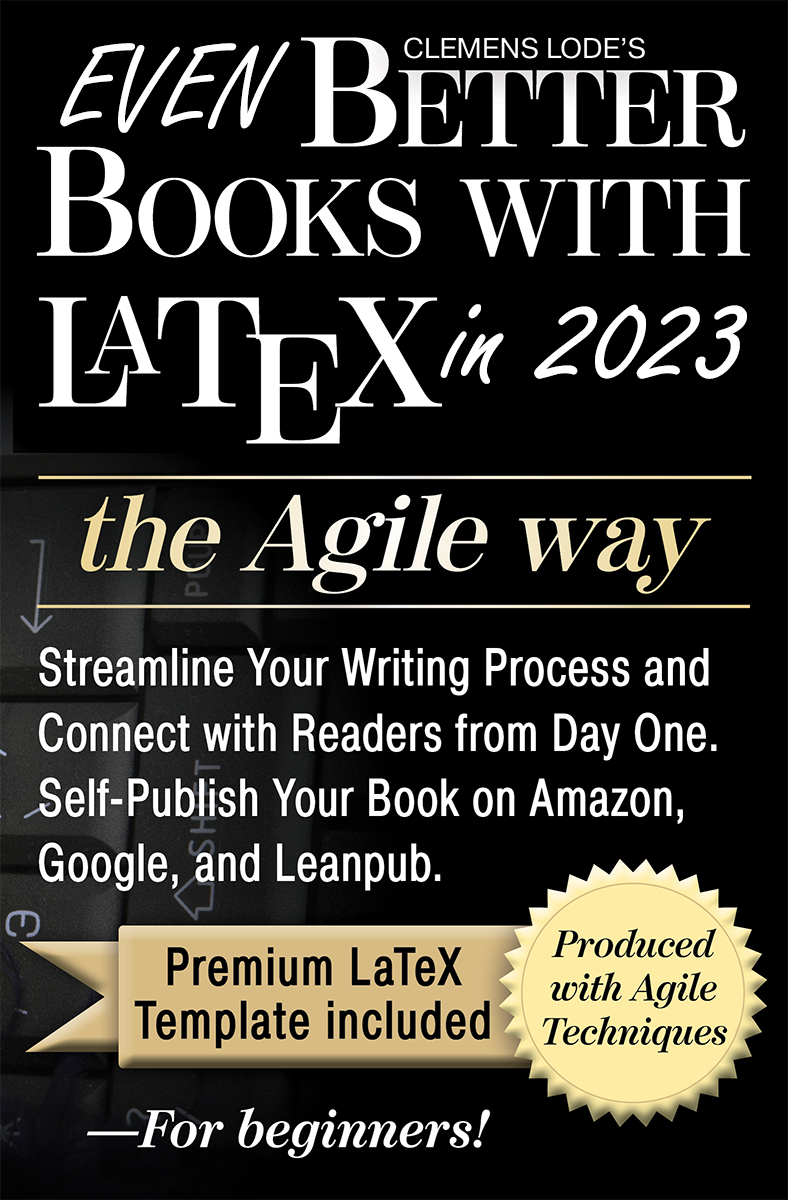
\includegraphics[width=.45\textwidth]{images/cover.jpg}
\end{center}

At LODE Publishing, we also publish works on science, philosophy, and project management. Check out \url{https://www.lode.de/publications} for a list. If you are interested in working with us to publish your book or if you are seeking advice on the next steps to take, contact us at \textbf{mail@lode.de}.\blankpage
% %%%%%%%%%%%%%%%%%%%%%%%%%%%%%%%%%%%%% 
% Check out the accompanying book, Even Better Books with LaTeX the Agile Way in 2023, for a discussion of the template and step-by-step instructions. https://amzn.to/3HqwgXM https://leanpub.com/eBBwLtAW/
% The template was originally created by Clemens Lode, LODE Publishing (www.lode.de), on 1/1/2023. Feel free to use this template for your book project! 
% I would be happy if you included a short mention in your book in order to help others to create their own books, too ("Book template based on \textit{Even Better Books with LaTeX the Agile Way in 2023} by Clemens Lode").
% Contact me at mail@lode.de if you need help with the template or are interested in our editing and publishing services.
% And don't forget to follow us on Instagram! https://www.instagram.com/lodepublishing/ https://www.instagram.com/betterbookswithlatex/
%%%%%%%%%%%%%%%%%%%%%%%%%%%%%%%%%%%%%

% This file prints the author page.

% Upload a high-resolution (author_highres.png) and a low-resolution picture (author.jpg) of the author into the images folder and uncomment the 5 includegraphics lines.
% Replace the paragraph about quotations with a quotation of your choice.
% Add text describing your motivation, your professional background, what you are currently doing, and how to connect with you.

\chapter{The Author \yourName}\label{the-author:cha}

\begin{center}

\ifuseAuthorImage
\ifxetex
	\includegraphics[width=.7\textwidth]{\authorImageHiRes}
\else
	\includegraphics{\authorImage}
\fi
\fi

\end{center}

\begin{myquotation} Here is space for a quotation that describes your journey through life (as opposed to just during the writing of this book). Pick one that best describes you, your attitude, or something you admire. Be personal!\end{myquotation}


Describe your dreams, what goals you have in life, where you went to school or studied, and what job you currently work or worked in the past. Make clear what motivated you to start writing. Finally, add contact points where people can connect with you (mail, Facebook, Instagram, TikTok, YouTube, Twitter, etc.). 
\blankpage
% %%%%%%%%%%%%%%%%%%%%%%%%%%%%%%%%%%%%% 
% Check out the accompanying book, Even Better Books with LaTeX the Agile Way in 2023, for a discussion of the template and step-by-step instructions. https://amzn.to/3HqwgXM https://leanpub.com/eBBwLtAW/
% The template was originally created by Clemens Lode, LODE Publishing (www.lode.de), on 1/1/2023. Feel free to use this template for your book project! 
% I would be happy if you included a short mention in your book in order to help others to create their own books, too ("Book template based on \textit{Even Better Books with LaTeX the Agile Way in 2023} by Clemens Lode").
% Contact me at mail@lode.de if you need help with the template or are interested in our editing and publishing services.
% And don't forget to follow us on Instagram! https://www.instagram.com/lodepublishing/ https://www.instagram.com/betterbookswithlatex/
%%%%%%%%%%%%%%%%%%%%%%%%%%%%%%%%%%%%%

% Use this chapter to summarize what you have learned while writing the book. This helps you to write better books in the future, and it might be interesting for the reader to learn how the book came about.

\chapter{The Book's Story}\label{booksstory:cha}

% Add a quotation that encompasses or describes the lessons you learned while planning and writing the book.



\blankpage
% %%%%%%%%%%%%%%%%%%%%%%%%%%%%%%%%%%%%% 
% Check out the accompanying book, Even Better Books with LaTeX the Agile Way in 2023, for a discussion of the template and step-by-step instructions. https://amzn.to/3HqwgXM https://leanpub.com/eBBwLtAW/
% The template was originally created by Clemens Lode, LODE Publishing (www.lode.de), on 1/1/2023. Feel free to use this template for your book project! 
% I would be happy if you included a short mention in your book in order to help others to create their own books, too ("Book template based on \textit{Even Better Books with LaTeX the Agile Way in 2023} by Clemens Lode").
% Contact me at mail@lode.de if you need help with the template or are interested in our editing and publishing services.
% And don't forget to follow us on Instagram! https://www.instagram.com/lodepublishing/ https://www.instagram.com/betterbookswithlatex/
%%%%%%%%%%%%%%%%%%%%%%%%%%%%%%%%%%%%%

\chapter{Reflection}

\begin{problem}
Introductory text about what this section is about. For example, describe that this is a summary of all the ``problem boxes'' throughout the book and point to an online forum where readers can discuss them.\end{problem}

% If you would like to reset formatting, use this code.
\setlength{\parindent}{0.0cm}
\renewcommand{\index}[1]{}
\renewenvironment{problem}[1][]{$\bullet$\ #1}
\footnotesize 


\section*{Replace with Your First Chapter}
% Add questions encountered in your first chapter.
\begin{definition}{LaTeX}\index{latex|textbf} LaTeX is a document preparation system.\end{definition}

\section*{Replace with Your Second Chapter}
% Add questions encountered in your second chapter.

\section*{Replace with Your Third Chapter}
% Add questions encountered in your third chapter.\blankpage
% \index{XeLaTeX@\textit{XeLaTeX}|textbf}
% %%%%%%%%%%%%%%%%%%%%%%%%%%%%%%%%%%%%% 
% Check out the accompanying book, Even Better Books with LaTeX the Agile Way in 2023, for a discussion of the template and step-by-step instructions. https://amzn.to/3HqwgXM https://leanpub.com/eBBwLtAW/
% The template was originally created by Clemens Lode, LODE Publishing (www.lode.de), on 1/1/2023. Feel free to use this template for your book project! 
% I would be happy if you included a short mention in your book in order to help others to create their own books, too ("Book template based on \textit{Even Better Books with LaTeX the Agile Way in 2023} by Clemens Lode").
% Contact me at mail@lode.de if you need help with the template or are interested in our editing and publishing services.
% And don't forget to follow us on Instagram! https://www.instagram.com/lodepublishing/ https://www.instagram.com/betterbookswithlatex/
%%%%%%%%%%%%%%%%%%%%%%%%%%%%%%%%%%%%%

% This file summarizes the conclusions or summaries of each chapter.

\chapter{Eureka!}

\begin{idea}
Introductory text about what this section is about. For example, describe that this is a summary of all the idea boxes throughout the book.\end{idea}

% Use the following command to reformat idea boxes.
\renewenvironment{idea}[1][]{$\bullet$\ #1}

% Use the following command to deactivate the indexing of idea boxes in order to prevent duplicates.
\ifxetex
        \renewcommand{\index}[1]{\ignorespaces}
\fi

\section*{Replace with Your First Chapter}
% Here, you can add ideas presented in your first chapter.
\begin{definition}{LaTeX}\index{latex|textbf} LaTeX is a document preparation system.\end{definition}

\section*{Replace with Your Second Chapter}
% Here, you can add ideas presented in your second chapter.

\section*{Replace with Your Third Chapter}
% Here, you can add ideas presented in your third chapter.\blankpage
% \index{XeLaTeX@\textit{XeLaTeX}|textbf}
% %%%%%%%%%%%%%%%%%%%%%%%%%%%%%%%%%%%%% 
% Check out the accompanying book, Even Better Books with LaTeX the Agile Way in 2023, for a discussion of the template and step-by-step instructions. https://amzn.to/3HqwgXM https://leanpub.com/eBBwLtAW/
% The template was originally created by Clemens Lode, LODE Publishing (www.lode.de), on 1/1/2023. Feel free to use this template for your book project! 
% I would be happy if you included a short mention in your book in order to help others to create their own books, too ("Book template based on \textit{Even Better Books with LaTeX the Agile Way in 2023} by Clemens Lode").
% Contact me at mail@lode.de if you need help with the template or are interested in our editing and publishing services.
% And don't forget to follow us on Instagram! https://www.instagram.com/lodepublishing/ https://www.instagram.com/betterbookswithlatex/
%%%%%%%%%%%%%%%%%%%%%%%%%%%%%%%%%%%%%

% This file lists the glossary items throughout the book.

% If you have added or removed any entries in the glossary directory, add them here. If a letter is missing, add a new \section*{} with the letter.

\chapter{Glossary}\label{glossary:cha}

\section*{C}
\begin{multicols}{2}
\babelEN{\begin{definition}{Citavi} \textit{Citavi} is a plugin for Word (see \url{https://www.citavi.com}) to manage your bibliography and citations.\end{definition}}\index{Citavi@\textit{Citavi}|textbf}
\end{multicols}

\section*{L}
\begin{multicols}{2}
\begin{definition}{LaTeX}\index{latex|textbf} LaTeX is a document preparation system.\end{definition}
\end{multicols}

\section*{O}
\begin{multicols}{2}
\babelEN{\begin{definition}{Overleaf} \textit{Overleaf} is an online editor and project manager for LaTeX documents. It manages your project with a versioning system and automatically compiles your LaTeX code into PDF and (with some help) HTML. It is free for public projects and does not require installation or setup. You can get an account here: \url{https://www.overleaf.com}.\end{definition}}\index{Overleaf@\textit{Overleaf}|textbf}

\end{multicols}

\section*{P}
\begin{multicols}{2}
\begin{definition}{pdfLaTeX} \textit{pdfLaTeX} is a basic LaTeX typesetting engine that translates LaTeX documents directly into PDFs or HTML files (with the help of \textit{TeX4ht}).\end{definition}\index{pdfLaTeX@\textit{pdfLaTeX}|textbf}
\end{multicols}

\section*{V}
\begin{multicols}{2}
\begin{definition}{Versioning system} A \textit{versioning system} is a tool to track changes to a document. That means you can go back and check what has been changed and by whom.\end{definition}\index{versioning system|textbf}
\end{multicols}

\section*{W}
\begin{multicols}{2}
\begin{definition}{Word} \textit{Word} usually refers to \textit{Microsoft Word}. Generally, it is used as an umbrella term for all word processors that directly show you what you will get as an end result (as opposed to first having to process the file). This approach is intuitive, but it makes editing large projects very complicated.\end{definition}\index{Word@\textit{Word}|textbf}
\end{multicols}

\section*{X}
\begin{multicols}{2}
\begin{definition}{XeLaTeX} \textit{XeLaTeX} is a LaTeX typesetting engine with an extended font, as well as UTF-8 encoding (for special characters) support. It takes longer to compile with \textit{XeLaTeX} than with the more basic \textit{pdfLaTeX}.\end{definition}\index{XeLaTeX@\textit{XeLaTeX}|textbf}




\end{multicols}\blankpage

% This adds a separate quotations page (sources in the e-book are already included in the text body).
\ifxetex
    %%%%%%%%%%%%%%%%%%%%%%%%%%%%%%%%%%%%% 
% Check out the accompanying book, Even Better Books with LaTeX the Agile Way in 2023, for a discussion of the template and step-by-step instructions. https://amzn.to/3HqwgXM https://leanpub.com/eBBwLtAW/
% The template was originally created by Clemens Lode, LODE Publishing (www.lode.de), on 1/1/2023. Feel free to use this template for your book project! 
% I would be happy if you included a short mention in your book in order to help others to create their own books, too ("Book template based on \textit{Even Better Books with LaTeX the Agile Way in 2023} by Clemens Lode").
% Contact me at mail@lode.de if you need help with the template or are interested in our editing and publishing services.
% And don't forget to follow us on Instagram! https://www.instagram.com/lodepublishing/ https://www.instagram.com/betterbookswithlatex/
%%%%%%%%%%%%%%%%%%%%%%%%%%%%%%%%%%%%%

% This file adds a page with quotation sources you have used in your book.

% This is displayed only for print PDFs where the source is not directly mentioned in the text body.

\chapter{Quotation Sources}

\setlength{\parindent}{0pt}
\footnotesize

\babelDE{\textbf{\pageref{gogh-sky-quote}:} \cite[vgl.][S.~23--24]{ifyouwanttowrite}}
\babelEN{\textbf{\pageref{gogh-sky-quote}:} \cite[pp.~23--24]{ifyouwanttowrite}}\par\blankpage
\fi

%%%%%%%%%%%%%%%%%%%%%%%%%%%%%%%%%%%%% 
% Check out the accompanying book, Even Better Books with LaTeX the Agile Way in 2023, for a discussion of the template and step-by-step instructions. https://amzn.to/3HqwgXM https://leanpub.com/eBBwLtAW/
% The template was originally created by Clemens Lode, LODE Publishing (www.lode.de), on 1/1/2023. Feel free to use this template for your book project! 
% I would be happy if you included a short mention in your book in order to help others to create their own books, too ("Book template based on \textit{Even Better Books with LaTeX the Agile Way in 2023} by Clemens Lode").
% Contact me at mail@lode.de if you need help with the template or are interested in our editing and publishing services.
% And don't forget to follow us on Instagram! https://www.instagram.com/lodepublishing/ https://www.instagram.com/betterbookswithlatex/
%%%%%%%%%%%%%%%%%%%%%%%%%%%%%%%%%%%%%

% This file prints the bibliography.

%  Uncomment the command below if you want to add a preface to the bibliography (between the title and the list of referenced books). See https://tex.stackexchange.com/questions/197061/text-between-index-or-bibliography-title-and-content

%\bibpreface {Add the preface of your list of recommended reading titles here. Delete this line to have no preface for this section.}

\ifxetex
    \printbibliography
\else
    \bibliographystyle{plainnat}
    \babelDE{\bibliography{chapters/bibliography/german}}
    \babelEN{\bibliography{chapters/bibliography/english}} 
\fi
\blankpage

%%%%%%%%%%%%%%%%%
% Appendix
%%%%%%%%%%%%%%%%%
\appendix

% The index page exists only for printed PDFs.
\ifxetex
    % This is an optional command to display a prologue before the index.
    % \indexprologue{Replace index prologue with an own introduction (errata, formatting, abbreviations, etc.).}
    
    \printindex\blankpage
    \thispagestyle{empty}
\fi

%%%%%%%%%%%%%%%%%%%%%%%%%%%%%%%%%%%%% 
% Check out the accompanying book, Even Better Books with LaTeX the Agile Way in 2023, for a discussion of the template and step-by-step instructions. https://amzn.to/3HqwgXM https://leanpub.com/eBBwLtAW/
% The template was originally created by Clemens Lode, LODE Publishing (www.lode.de), on 1/1/2023. Feel free to use this template for your book project! 
% I would be happy if you included a short mention in your book in order to help others to create their own books, too ("Book template based on \textit{Even Better Books with LaTeX the Agile Way in 2023} by Clemens Lode").
% Contact me at mail@lode.de if you need help with the template or are interested in our editing and publishing services.
% And don't forget to follow us on Instagram! https://www.instagram.com/lodepublishing/ https://www.instagram.com/betterbookswithlatex/
%%%%%%%%%%%%%%%%%%%%%%%%%%%%%%%%%%%%%

% This file adds a page reminding the reader to leave a review.

% Replace this with your own call to action or use the default text.
\chapter{An Important Final Note}

% Show this paragraph only for e-books.
\ifxetex \else \textit{If you want to rate this e-book, please also add a short text comment. Without a text comment, your star rating will be invisible on the Amazon website and count only as an indicator for additional recommendations on Amazon. Thanks!}\fi

% Show the following for e-books and printed books. 
Writers are not performance artists. While there are book signings and public readings, most writers (and readers) follow their passion alone in their homes.

\textit{What applause is for the musician, \textbf{reviews} are for the writer.} 

\textit{Books create a community among readers}; you can share your thoughts among all those who will or have read the book.

\textbf{Leave a thoughtful, honest review and help me to create such a community on the platform on which you have acquired this book.} 
\textit{What did you like, what can be improved? To whom would you recommend it?} 

Thank you, also in the name of all the other readers who will be able to better decide whether this book is right for them or not. A positive review will increase the reach of the book; a negative review will improve the quality of the next book. I welcome both!\blankpage
%%%%%%%%%%%%%%%%%%%%%%%%%%%%%%%%%%%%% 
% Check out the accompanying book, Even Better Books with LaTeX the Agile Way in 2023, for a discussion of the template and step-by-step instructions. https://amzn.to/3HqwgXM https://leanpub.com/eBBwLtAW/
% The template was originally created by Clemens Lode, LODE Publishing (www.lode.de), on 1/1/2023. Feel free to use this template for your book project! 
% I would be happy if you included a short mention in your book in order to help others to create their own books, too ("Book template based on \textit{Even Better Books with LaTeX the Agile Way in 2023} by Clemens Lode").
% Contact me at mail@lode.de if you need help with the template or are interested in our editing and publishing services.
% And don't forget to follow us on Instagram! https://www.instagram.com/lodepublishing/ https://www.instagram.com/betterbookswithlatex/
%%%%%%%%%%%%%%%%%%%%%%%%%%%%%%%%%%%%%
% This file is the last page of the book.

\thispagestyle{empty}
\ifxetex
    \vspace*{\fill}
\fi
\hfill

% Replace the quote.
\babelEN{\begin{myquotation} Replace this quote\par\mbox{}\hfill \emdash{}Name of the author\end{myquotation}}

\end{document}